\documentclass[%
    % draft,%
    xcolor=usenames,dvipsnames,svgnames%
]{beamer}

% \setbeameroption{show notes}
% \setbeameroption{show only notes}

\RequirePackage{xparse}

%% https://www.quora.com/Presentations-What-are-the-best-beamer-themes
\setbeamertemplate{frametitle}
  {\begin{centering}\smallskip
   \insertframetitle\par
   \smallskip\end{centering}}
% https://tex.stackexchange.com/a/56541/94717
% https://tex.stackexchange.com/q/125540/94717
\makeatletter
\newcommand\listofframes{\@starttoc{lbf}}
\makeatother
\addtobeamertemplate{frametitle}{}{%
  \addcontentsline{lbf}{section}{\protect\makebox[2em][l]{%
    \protect\usebeamercolor[fg]{structure}\insertframenumber\hfill}%
  \insertframetitle\par}%
}
\setbeamertemplate{itemize item}{\(\bullet\)}
\setbeamertemplate{navigation symbols}{}
\setbeamertemplate{footline}[text line]{%
    \hfill\strut{%
        \scriptsize\sf\color{black!60}%
        \quad\insertframenumber
    }%
    \hfill
}
\setbeamertemplate{section in toc}[ball unnumbered]

\definecolor{NoteBrown}{RGB}{152,101,47}
\definecolor{NoteBlue}{RGB}{31,91,255}
\definecolor{NoteGreen}{RGB}{62,195,74}
\definecolor{NoteRed}{RGB}{191,0,0}
\definecolor{NotePurple}{RGB}{151,54,208}
\definecolor{NoteDarkGreen}{RGB}{0,121,62}
\definecolor{NoteGrey}{RGB}{150,150,150}
\definecolor{NoteOrange}{RGB}{255,155,0}

% Define some colors:
\definecolor{PittBlue}{RGB}{0,43,94}
\definecolor{PittGold}{RGB}{197,168,118}
\definecolor{DarkFern}{HTML}{407428}
\definecolor{DarkCharcoal}{HTML}{4D4944}
\colorlet{Fern}{DarkFern!85!white}
\colorlet{Charcoal}{DarkCharcoal!85!white}
\colorlet{LightCharcoal}{Charcoal!50!white}
\colorlet{AlertColor}{orange!80!black}
\colorlet{DarkRed}{red!70!black}
\colorlet{DarkBlue}{blue!70!black}
\colorlet{DarkGreen}{green!70!black}
% Use the colors:
\setbeamercolor{title}{fg=PittBlue}
\setbeamercolor{frametitle}{fg=PittBlue}
\setbeamercolor{normal text}{fg=DarkCharcoal}
\setbeamercolor{block title}{fg=black,bg=Fern!25!white}
\setbeamercolor{block body}{fg=black,bg=Fern!25!white}
\setbeamercolor{alerted text}{fg=AlertColor}
\setbeamercolor{itemize item}{fg=Charcoal}

\usepackage[%
    backend    = biber,%
    style      = chem-acs,%
    autocite   = superscript,%
    backref    = true,%
    biblabel   = brackets,%
    doi        = true,%
    minnames   = 1,%
    maxnames   = 10,%
]{biblatex}
\addbibresource{../library.bib}
\addbibresource{../library2.bib}
\addbibresource{../paper_04/paper.bib}
\addbibresource{../paper_05/psi4numpy.bib}
\addbibresource{../paper_05/tutorial.bib}
\addbibresource{../5746059.bib}
\addbibresource{../5773968.bib}
\addbibresource{../in_preparation.bib}
\addbibresource{./presentation.bib}

\AtEveryCitekey{\iffootnote{\color{PittBlue}\tiny}{}}
\NewDocumentCommand{\nmfootfullcite}{m}{%
    \AtNextCite{%
        \let\thefootnote\relax
        \let\mkbibfootnote\mkbibfootnotetext
    }{%
        \footfullcite{#1}
    }
}

\RequirePackage{appendixnumberbeamer}
\RequirePackage{booktabs}
\RequirePackage{braket}
\RequirePackage{caption}
\RequirePackage{graphicx}
\RequirePackage{microtype}
\RequirePackage{minted}
\RequirePackage[version=4]{mhchem}
\newcommand{\arlidimer}{\ce{Ar\bond{....}Li+}}
\RequirePackage[%
    separate-uncertainty = true,%
    multi-part-units = single,%
    range-units = single,%
    retain-explicit-plus = true,%
]{siunitx}
\RequirePackage{subcaption}
\RequirePackage{tabulary}

\NewDocumentCommand{\vect}{m}{%
        \ensuremath{\boldsymbol{\mathbf{#1}}}%
}%

% \newcommand*{\phnum}[2][]{%
%   \begingroup
%     \protected\def\X{\phantom{0}}%
%     \num[
%       input-digits=0123456789\X,%
%       #1%
%     ]{#2}%
%   \endgroup
% }

% https://tex.stackexchange.com/q/252586/94717
\newwrite\tempfile
\immediate\openout\tempfile=slidelist.txt
\newcounter{SlideNumber}
\addtobeamertemplate{frametitle}{}{%
  \stepcounter{SlideNumber}
  \immediate\write\tempfile{\theSlideNumber [\insertframenumber] \insertframetitle}
}

% \newcommand\pfour{\textsc{Psi4}}
\newcommand\pfour{Psi4}
% \newcommand\pfn{\textsc{Psi4NumPy}}
\newcommand\pfn{Psi4NumPy}

\title{Decomposition of Intermolecular Interactions in \textit{Ab Initio} Spectroscopy}
\author{Eric Berquist}
\institute{
\includegraphics[width=1in]{./figures/pitt_logo.pdf}}
\date{March 23th, 2018}

\begin{document}

\frame{
  \titlepage
}

\frame{
  \frametitle{Goal of this work}
  It is possible to identify the contribution of specific molecular interactions to spectroscopic response.
  \tableofcontents
}

\note{\tiny\listofframes}

\begin{frame}
  \frametitle{Spectroscopy is a probe of changes in a molecule's electronic and geometric state using electromagnetic radiation}
  \centering
  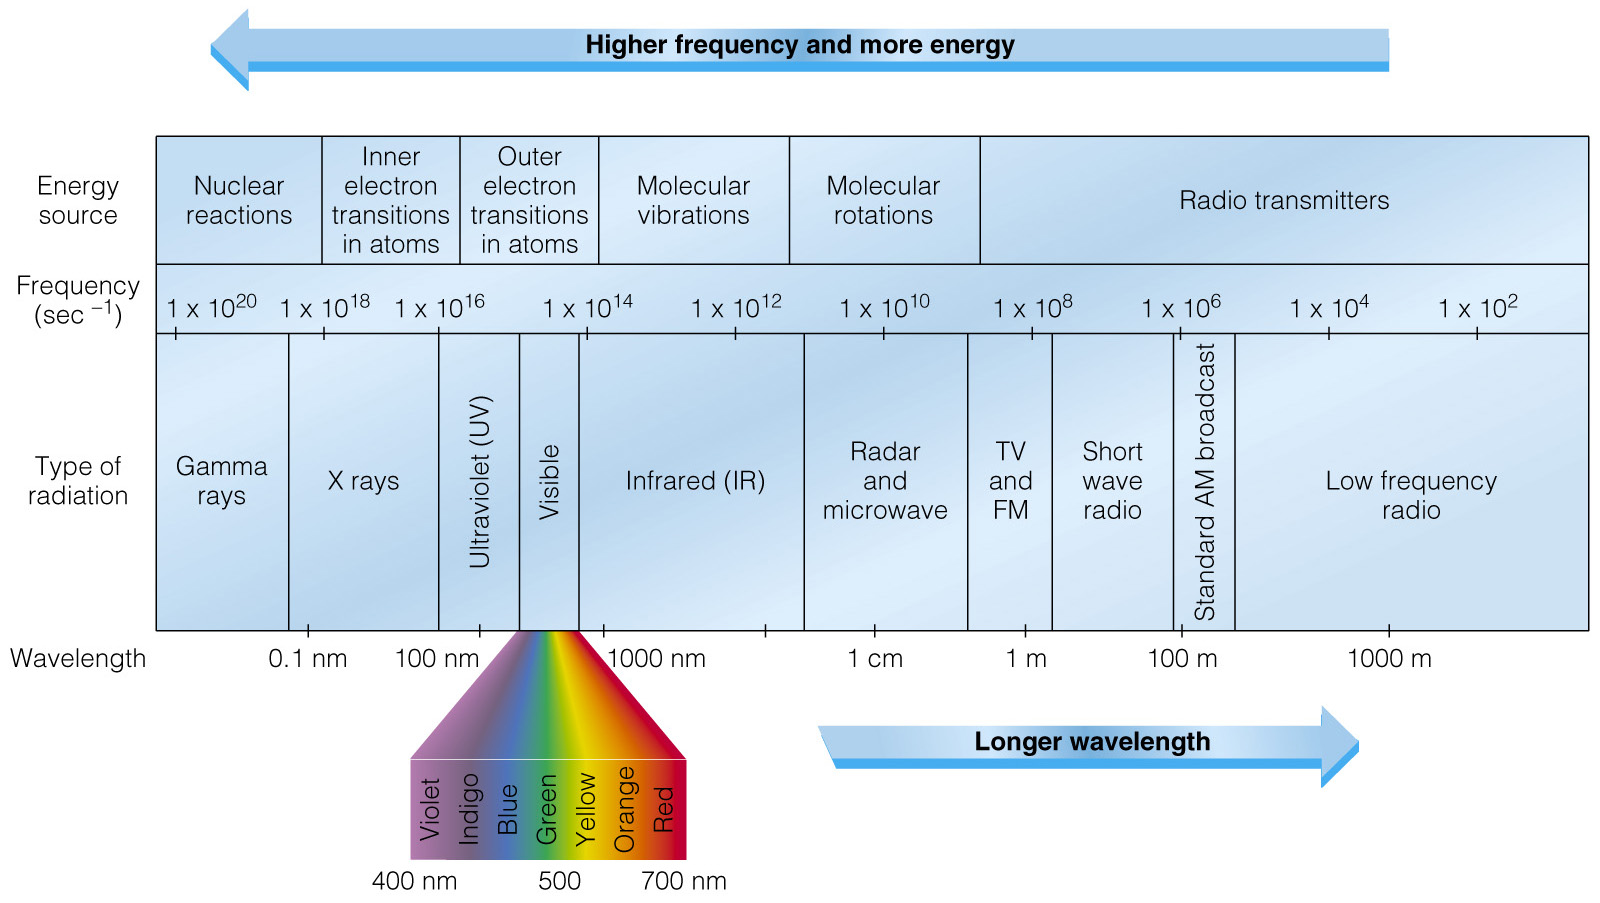
\includegraphics[width=\linewidth,keepaspectratio]{./figures/electromagnetic-spectrum.jpg}
  {\tiny\url{http://hrsbstaff.ednet.ns.ca/benoitn/chem11/units/1.\%20Atomic\%20Theory/e_config/spectra/electromagnetic-spectrum.jpg}}
  \note[item]{Tom comment: "not excited states, just looking at polarizability" -- this statement did not make sense to me}
  \note[item]{Response: wavelengths associated with frequency-dependent polarizability are also associated with UV/vis; probably don't need to mention this}
\end{frame}

\section{Decomposition of harmonic vibrational frequencies into physically-intuitive terms}

\begin{frame}[fragile]
  \frametitle{\protect{Infrared spectroscopy is sensitive to the presence of \ce{CO2} in ionic liquids}}
  \note[item]{For example, ...}
  \note[item]{FTIR IL spectra with and without CO2 goes here}
  % \frametitle{\ce{CO2} asymmetric stretch lies in an isolated spectral window}
  \centering
  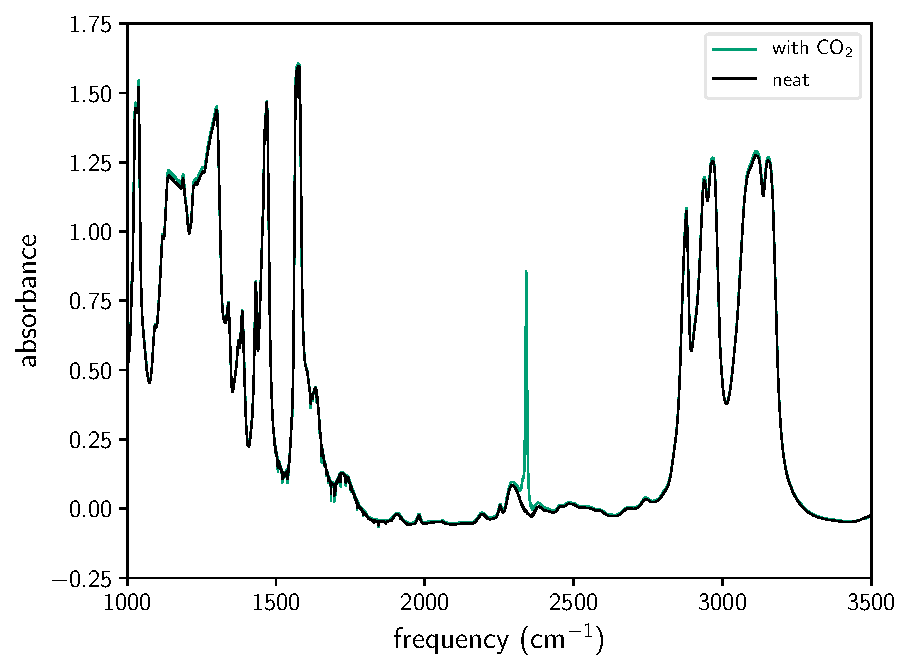
\includegraphics[width=\linewidth,keepaspectratio]{./figures/experimental_spectra_TfO.pdf}
\end{frame}

\begin{frame}[fragile]
  \frametitle{\protect{Understanding \ce{CO2} solvation by ionic liquids is important for carbon capture}}
  \note[item]{Lewis structures go here}
  \note[item]{Example ionic liquids for carbon capture}
  \note[item]{Why these? Water tolerant, fairly good CO2 capture already, experimentally studied/validated}
  \note[item]{desirable properties of ionic liquids: solvation energy, reversible absorption}
  \note[item]{point out nomenclature}
  \begin{figure}
    \centering
    \begin{subfigure}[b]{0.25\linewidth}
      \centering
      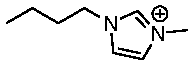
\includegraphics[scale=1.00]{./figures/lewis_C4C1im.pdf}
      \caption*{\ce{[C4C1im]+}}
    \end{subfigure}
    % \begin{subfigure}[b]{0.25\linewidth}
    %   \centering
    %   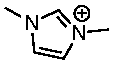
\includegraphics[scale=1.00]{./figures/lewis_C1C1im.pdf}
    %   \caption*{\ce{[C1C1im]+}}
    % \end{subfigure}
    \begin{subfigure}[b]{0.25\linewidth}
      \centering
      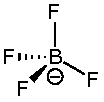
\includegraphics[scale=1.00]{./figures/lewis_BF4.pdf}
      \caption*{\ce{[BF4]-}}
    \end{subfigure}
    \begin{subfigure}[b]{0.25\linewidth}
      \centering
      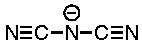
\includegraphics[scale=1.00]{./figures/lewis_DCA.pdf}
      \caption*{\ce{[DCA]-}}
    \end{subfigure}
    \begin{subfigure}[b]{0.25\linewidth}
      \centering
      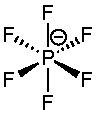
\includegraphics[scale=1.00]{./figures/lewis_PF6.pdf}
      \caption*{\ce{[PF6]-}}
    \end{subfigure}
    \begin{subfigure}[b]{0.25\linewidth}
      \centering
      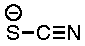
\includegraphics[scale=1.00]{./figures/lewis_SCN.pdf}
      \caption*{\ce{[SCN]-}}
    \end{subfigure}
    \begin{subfigure}[b]{0.25\linewidth}
      \centering
      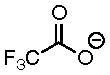
\includegraphics[scale=1.00]{./figures/lewis_TFA.pdf}
      \caption*{\ce{[TFA]-}}
    \end{subfigure}
    \begin{subfigure}[b]{0.25\linewidth}
      \centering
      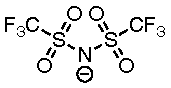
\includegraphics[scale=1.00]{./figures/lewis_Tf2N.pdf}
      \caption*{\ce{[Tf2N]-}}
    \end{subfigure}
    \begin{subfigure}[b]{0.25\linewidth}
      \centering
      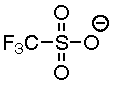
\includegraphics[scale=1.00]{./figures/lewis_TfO.pdf}
      \caption*{\ce{[TfO]-}}
    \end{subfigure}
  \end{figure}
\end{frame}

\begin{frame}
  \frametitle{Solvatochromic shift originates from varying the ionic liquid anion}
  \note[item]{shift as function of anion goes here}
  \centering
  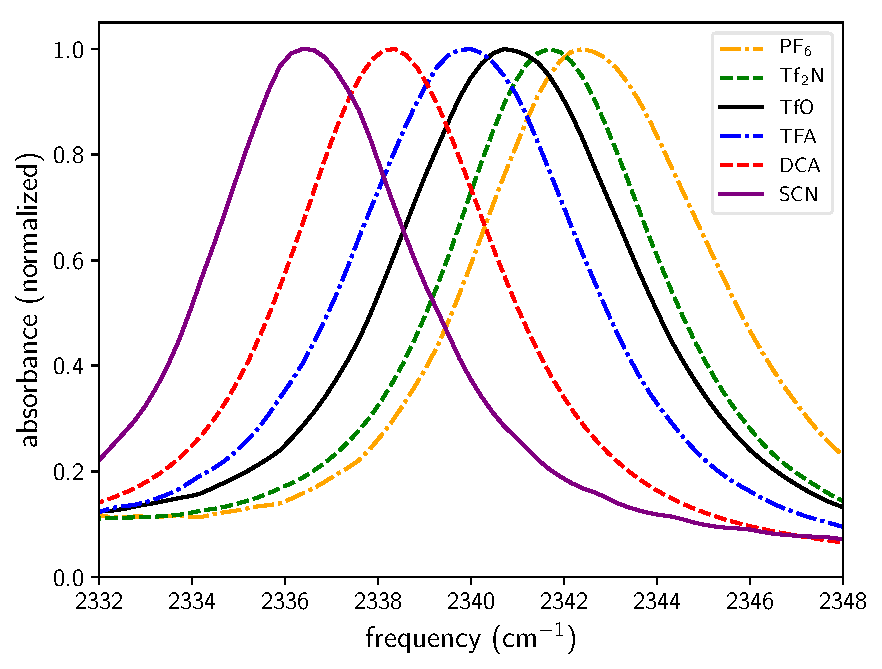
\includegraphics[scale=0.65]{./figures/experimental_spectra_shifting.pdf}
  \scriptsize
  experiment, \ce{[C4C1im]+}
\end{frame}

\begin{frame}
  \frametitle{Model calculations qualitatively reproduce trends in the solvatochromic shift}
  \note[item]{Experiment/calculation trends go here}
  \note[item]{Put image of TFA cluster in plot whitespace}
  \note[item]{Experimental cation is C4C1im, computational cation is C1C1im}
  \note[item]{quantum chemistry connects frequencies to structure}
  \centering
  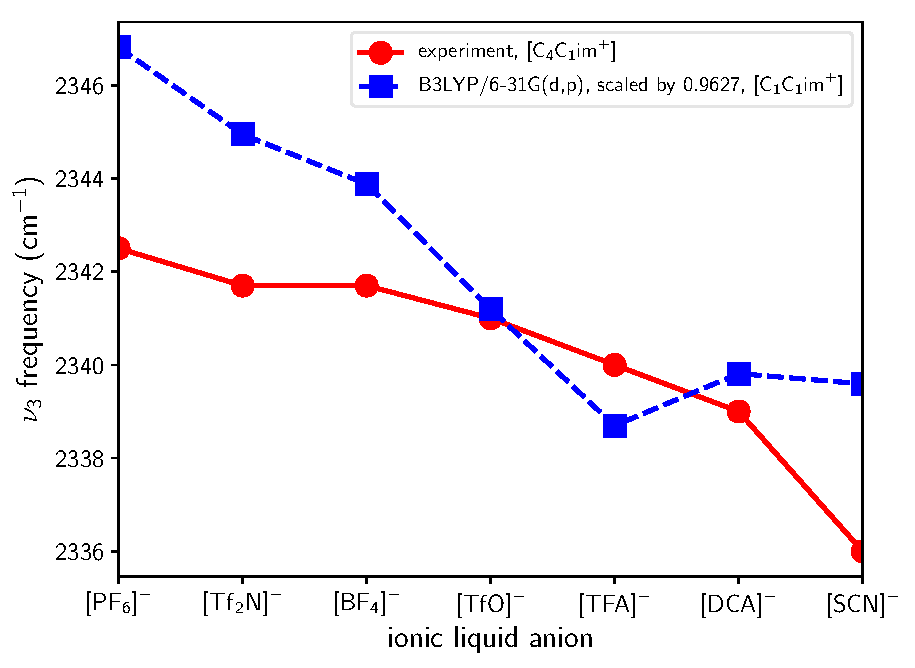
\includegraphics[width=\linewidth,keepaspectratio]{./figures/frequencies_calc_vs_expt1.pdf}
  % \nmfootfullcite{Brinzer2015}
\end{frame}

\begin{frame}
  % \frametitle{ALMO-EDA enables understanding the physical basis for the solvatochromic shift}
  \frametitle{What is the physical basis for the solvatochromic shift?}
\end{frame}

\begin{frame}
  \frametitle{Energy decomposition analysis provides an intuitive assignment of intermolecular interactions to physical terms}
  \note[item]{Performed using absolutely localized molecular orbitals (ALMO-EDA), a ``bottom-up'' localization technique that prevents charge transfer by construction}
  \note[item]{How an ALMO is constructed}
  \note[item]{Intermediate wavefunction!}
  \note[item]{Can move on the ALMO potential energy surface}
  \note[item]{Explanation of Pauli repulsion, signs of terms}
\end{frame}

\note{If going to talk about the geometry mechanism and the curvature mechanism, it should go here?}

\begin{frame}[fragile]
  \frametitle{\protect{The \ce{CO2} asymmetric stretch solvatochromic shift is caused by charge transfer-driven geometric distortion}}
  \begin{figure}
    \centering
    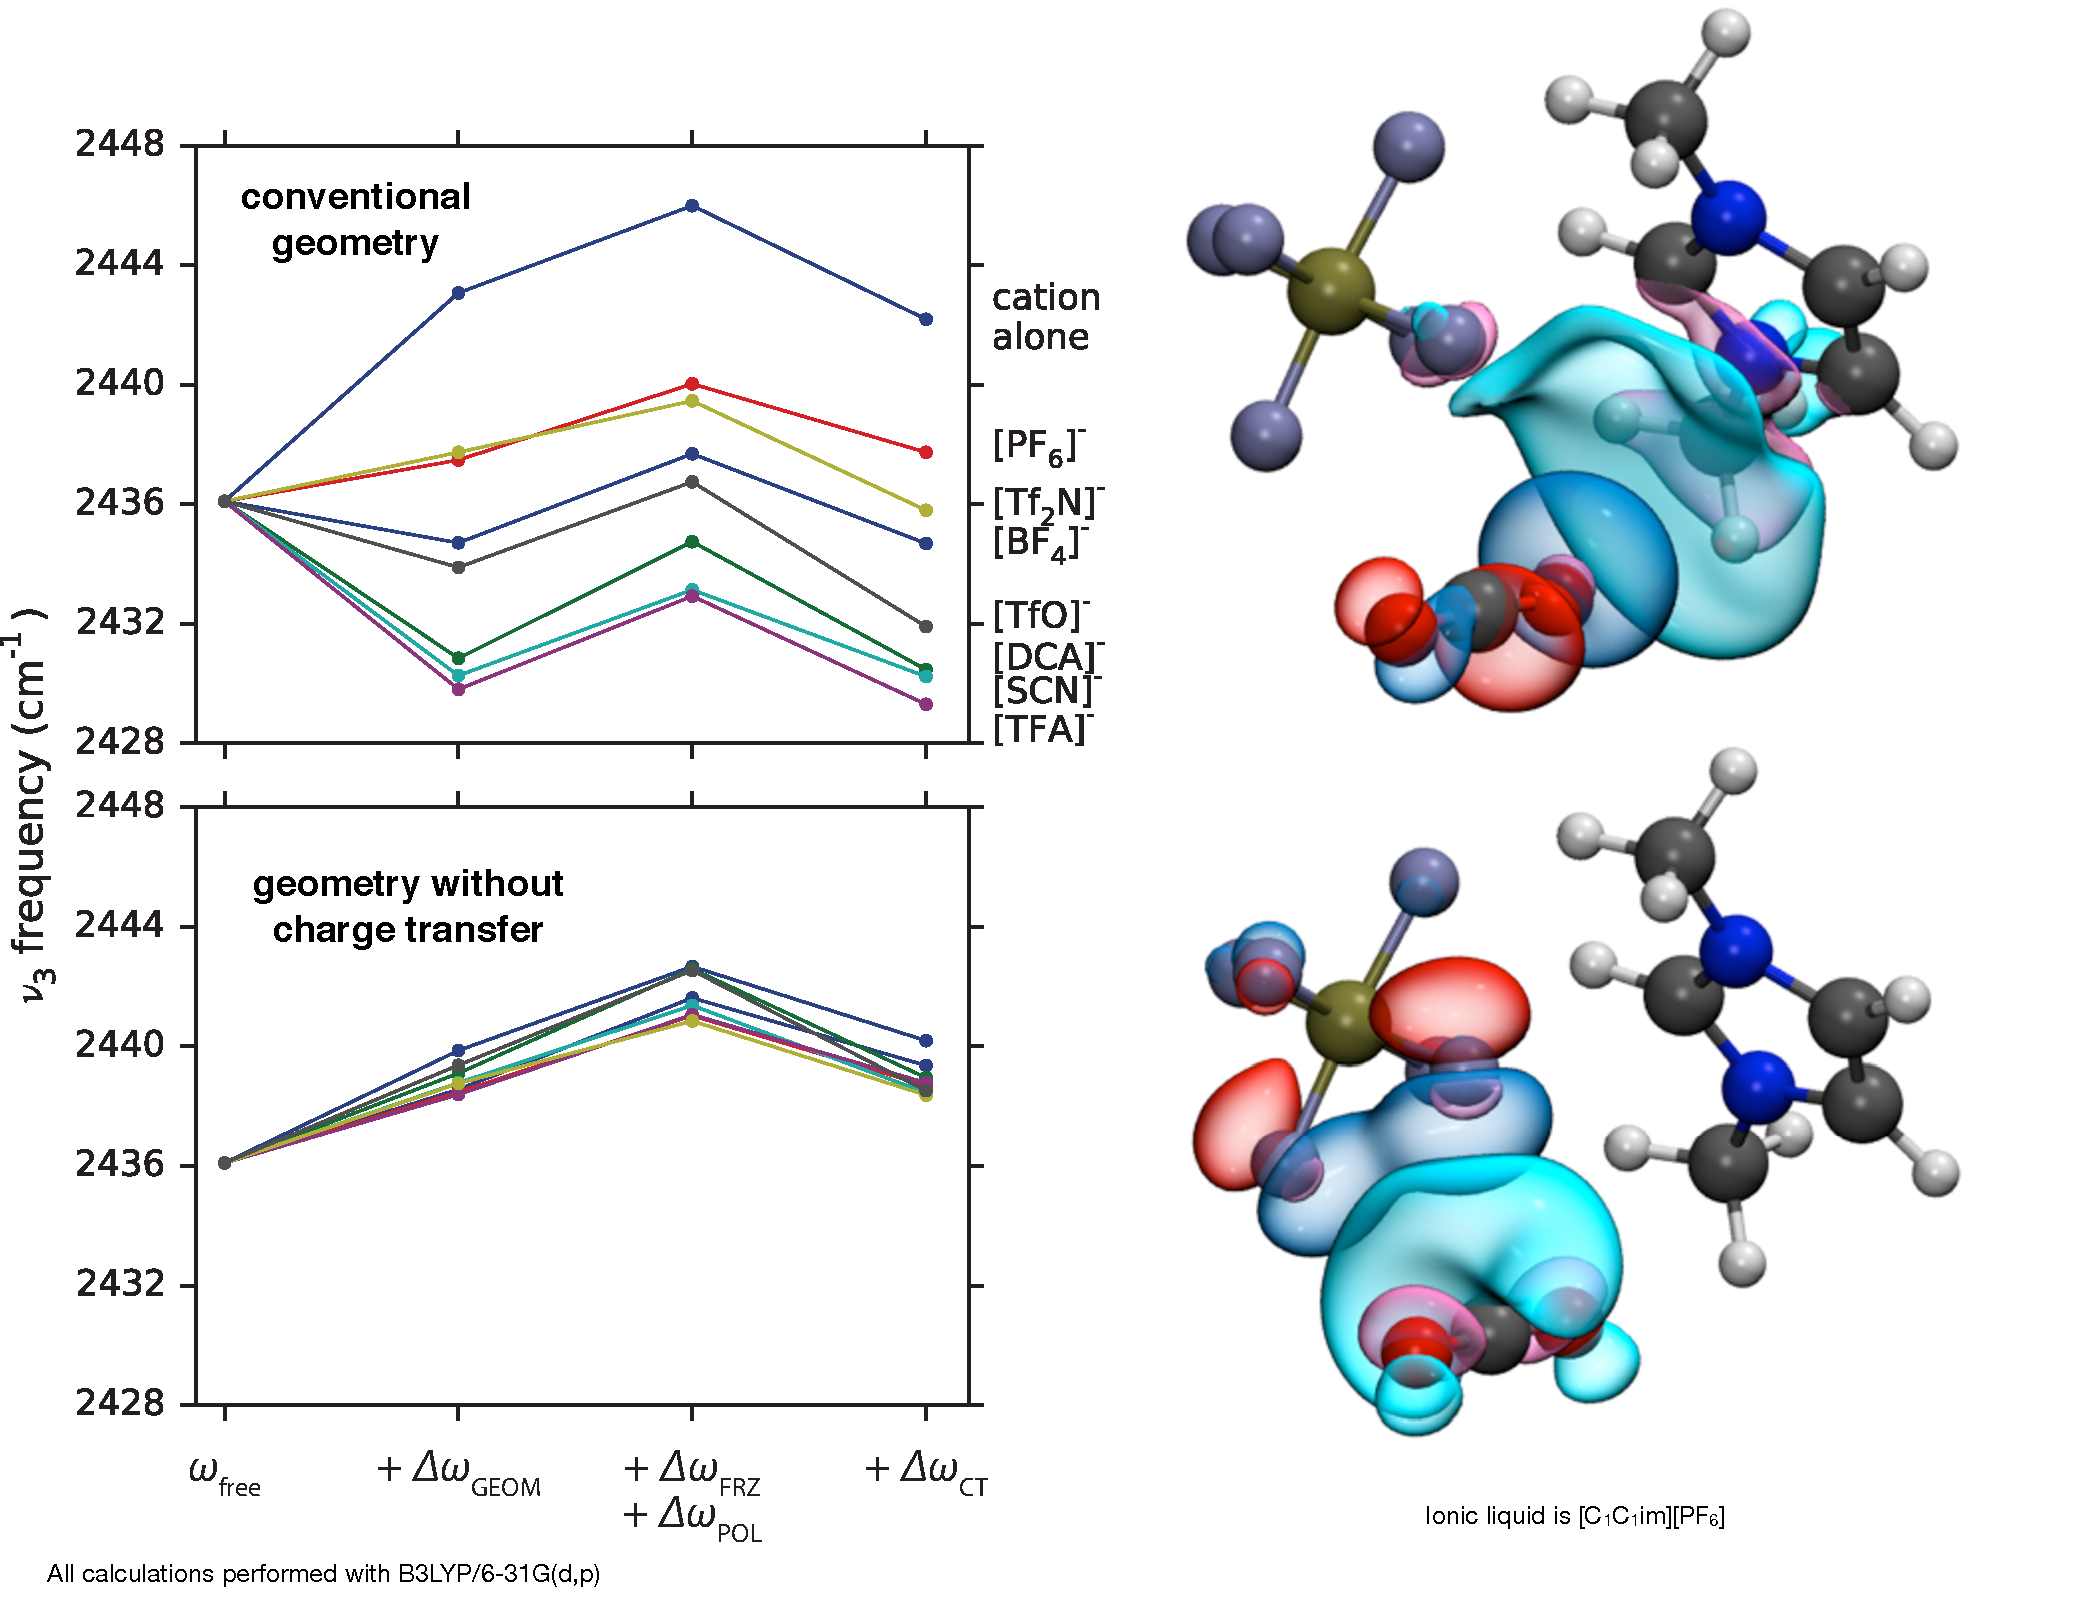
\includegraphics[scale=0.25]{./figures/ionic_liquid_geometry_dependence_on_ct_combined.pdf}
  \end{figure}
  % B3LYP/6-31G(d,p); cation is \ce{[C1C1im]+}
\end{frame}

\begin{frame}
  \frametitle{Conclusion: spectra decomposition is an integral part of the experimental-computational workflow}
  \note[item]{cite Daly papers}
  \begin{columns}
    \column{0.35\linewidth}
    I am a filler line
    \column{0.65\linewidth}
    % 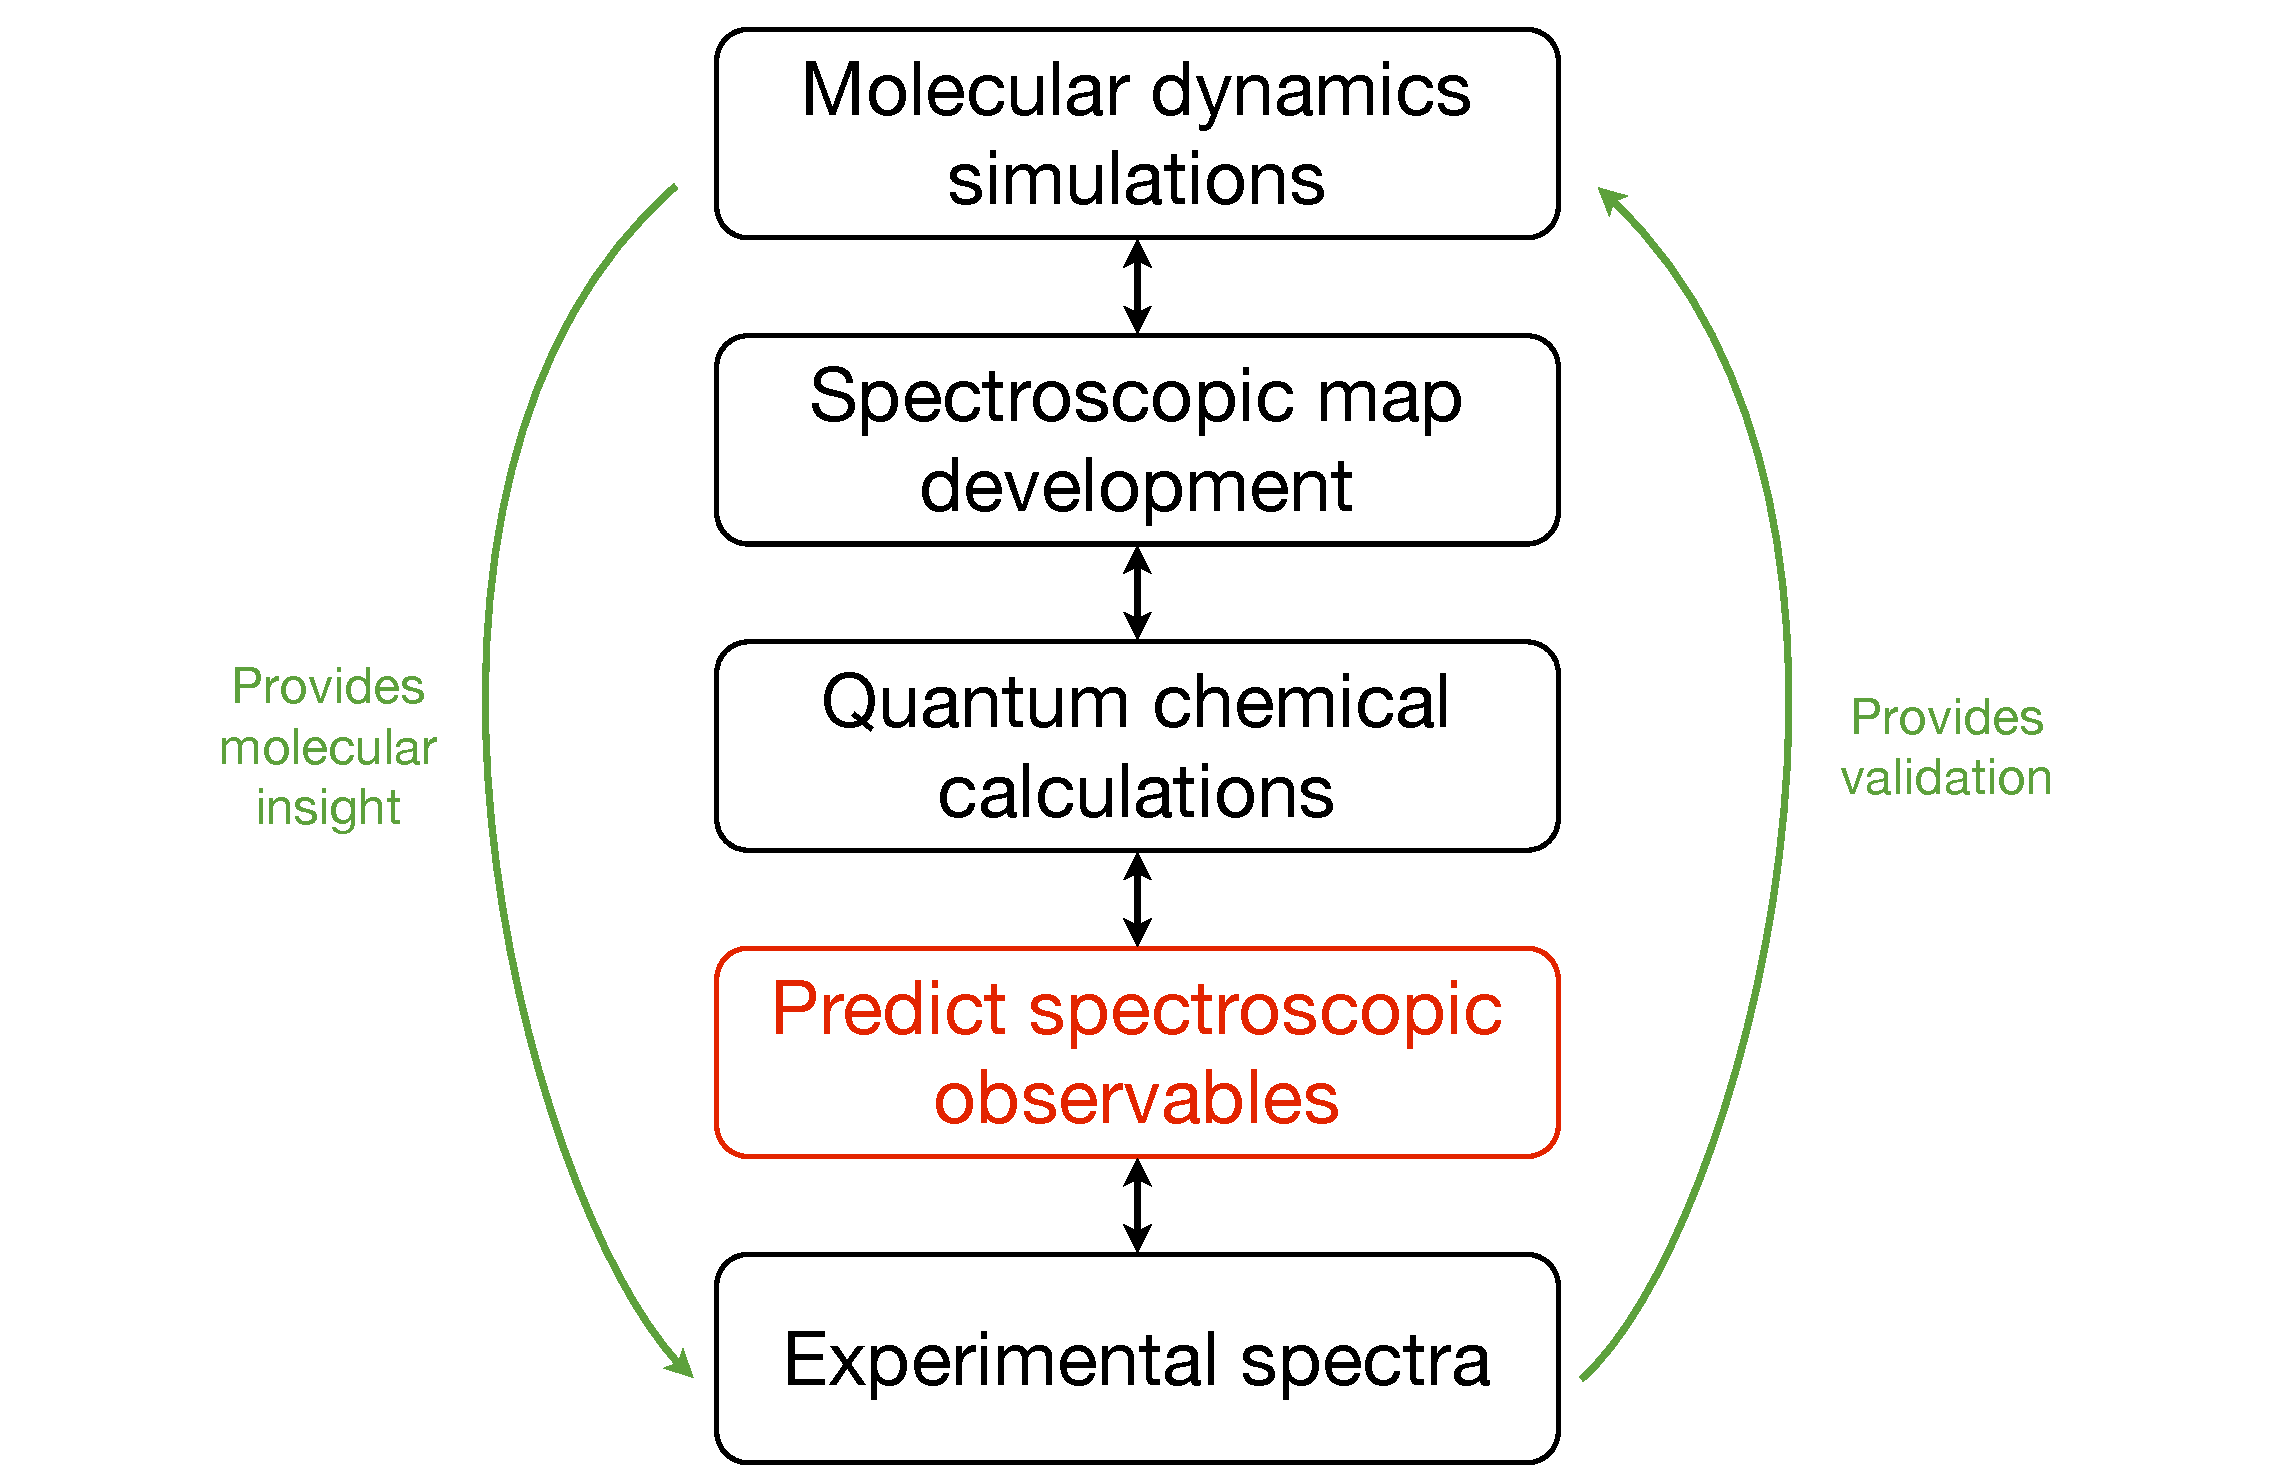
\includegraphics[scale=0.15]{./figures/workflow.pdf}
    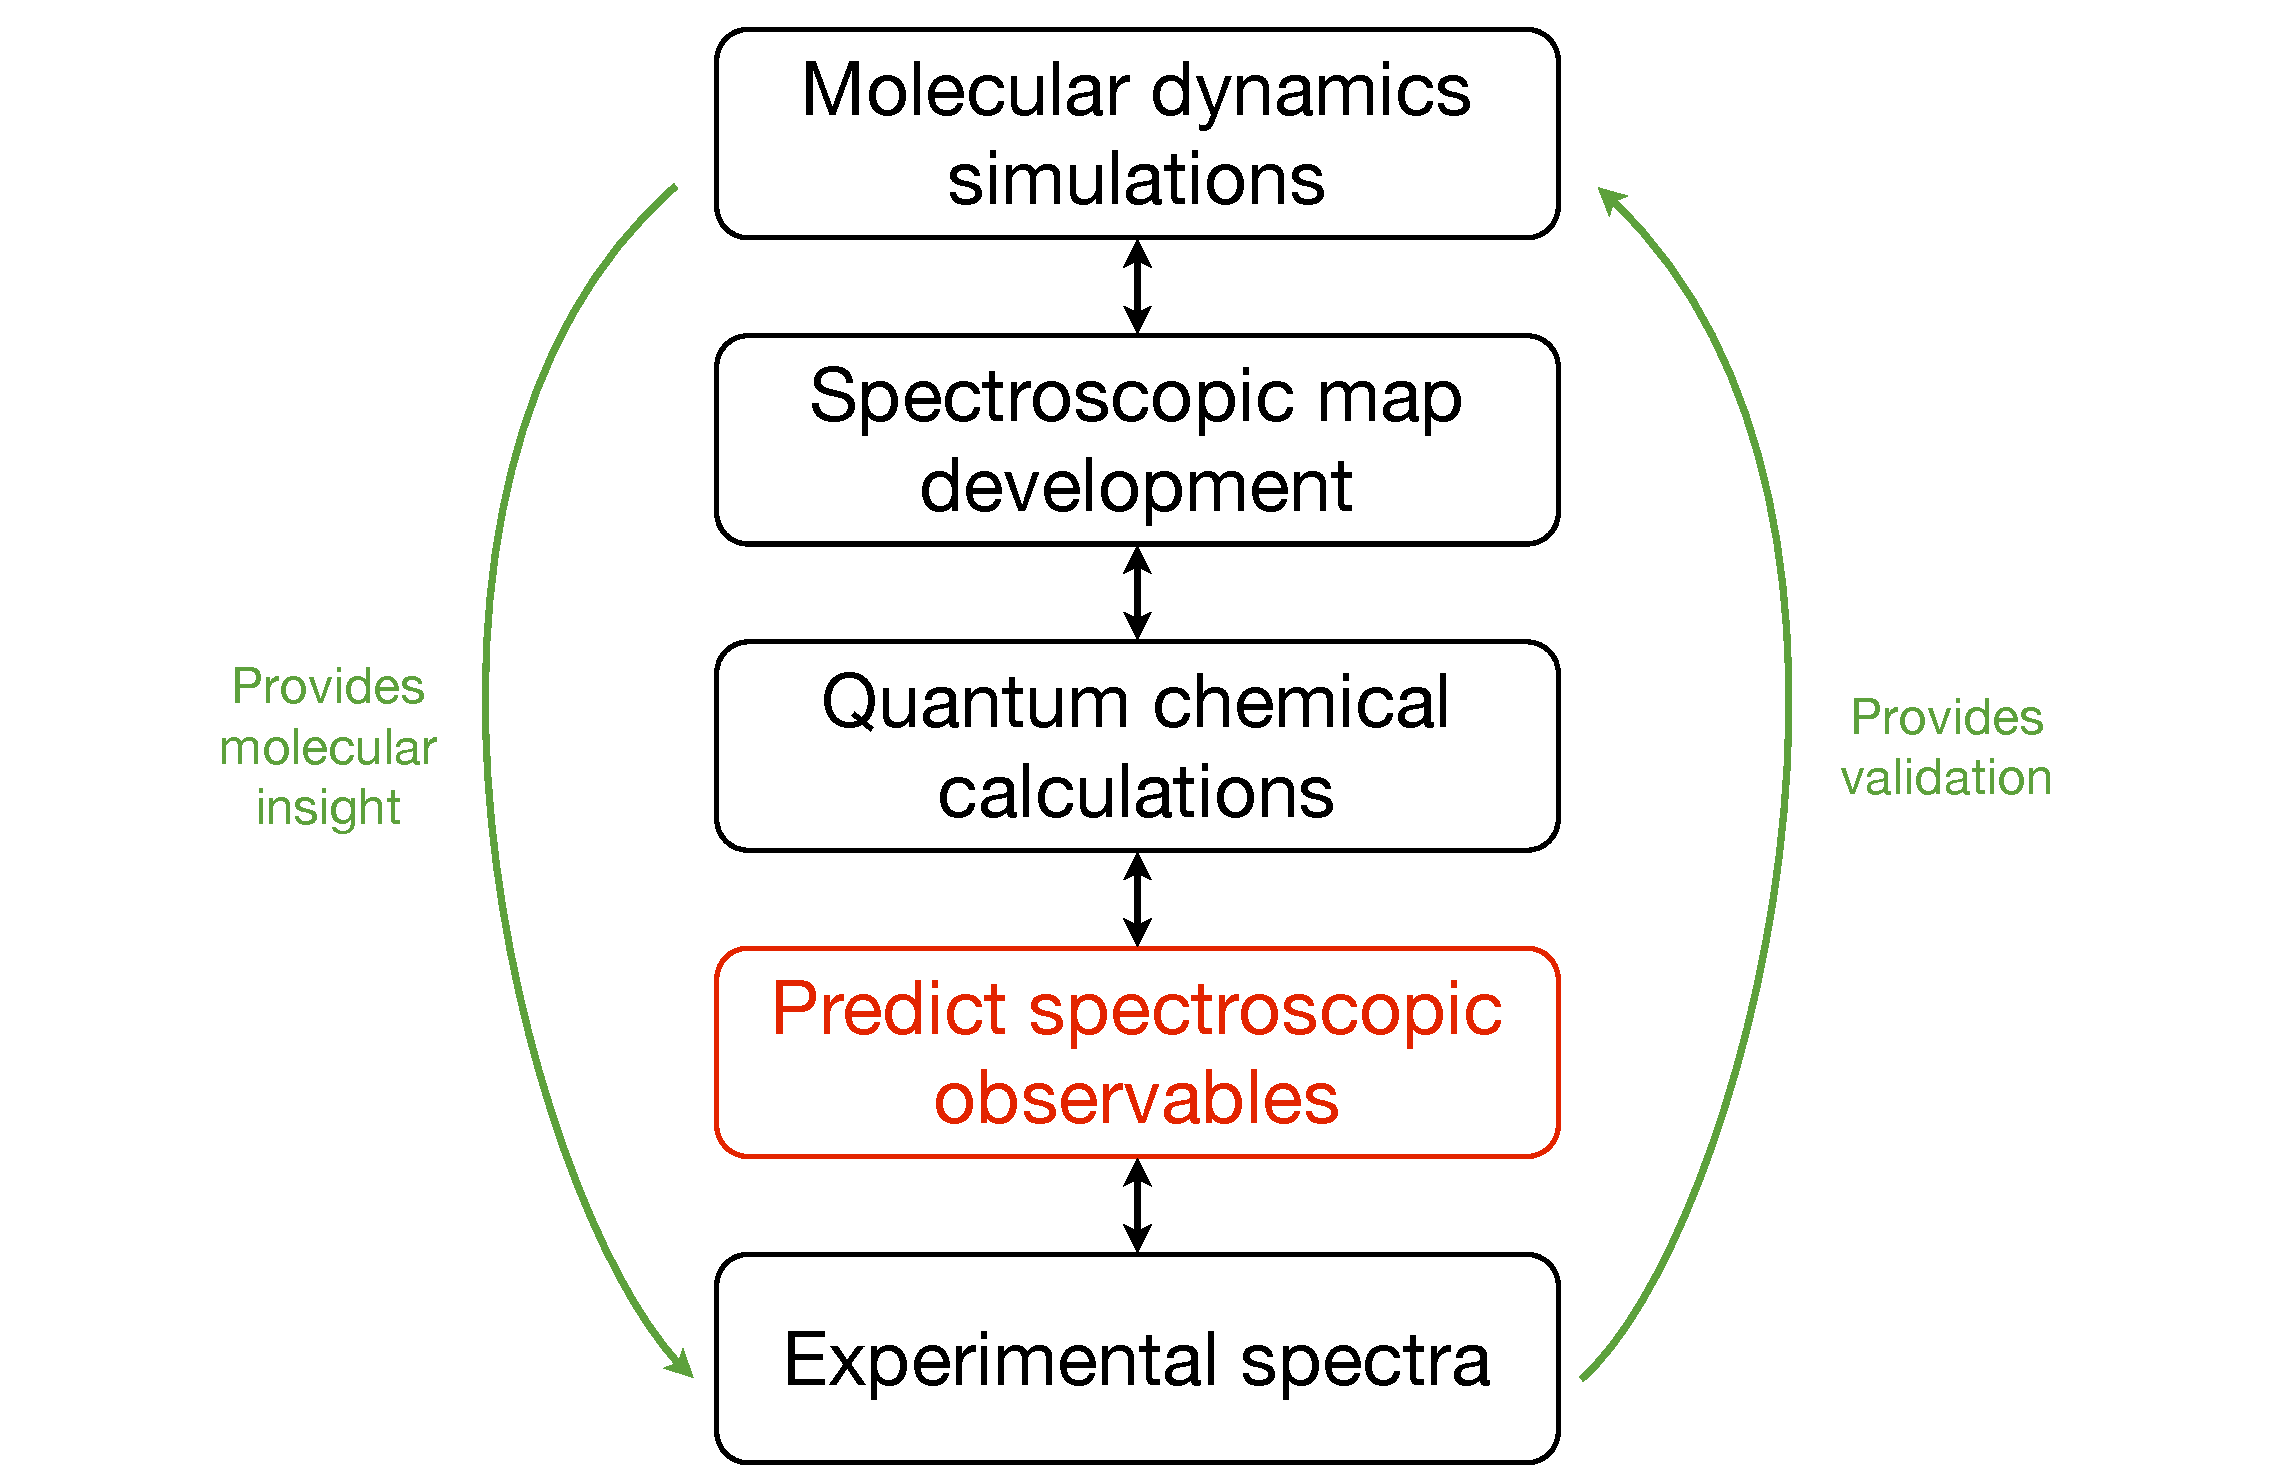
\includegraphics[width=\linewidth,keepaspectratio]{./figures/workflow.pdf}
  \end{columns}
\end{frame}

\begin{frame}
  \frametitle{Problem: the approach for decomposing vibrational frequencies is not generally applicable to other properties}
  \note[item]{What's the value of spectroscopy decomposition?}
  \note[item]{Want the ability to build structure-spectra relationships for any type of spectroscopy, leading to spectra-property relationships}
  \note[item]{A series expansion example + e-field terms should go here}
\end{frame}

\begin{frame}
  \frametitle{Spectroscopic properties are directly connected to energy derivatives}
  \note[item]{The derivative table should go here}
\end{frame}

\begin{frame}
  \frametitle{Numerical differentiation can give unphysical results}
  \note[item]{this is where the polarizability asymmetry figure goes}
  \note[item]{One example why the original approach is not generally applicable...}
  \note[item]{One problem with numerical differentiation is...}
  \note[item]{Mention other issues with numerical differentiation}
\end{frame}

\section{Decomposition of general linear response properties}

\begin{frame}
  \frametitle{Solution: start from the framework of response theory}
  \note[item]{Many important molecular properties are calculated within the framework of linear response}
  Spectroscopic properties are directly connected to (linear) response functions:
  \note[item]{the linear response table should go here}
  \note[item]{Linear response is named as such not due to the linear form of the equations, but because the perturbation is linear in strength. This strength may be constant, static, or time-independent, or it may be oscillating, dynamic, frequency-, or time-dependent.}
\end{frame}

\begin{frame}
  \frametitle{The language of energy decomposition analysis can be applied to general response properties}
  We have already successfully translated
  \begin{equation*}
    \Delta E_{\text{int}} = \Delta E_{\text{geom}} + \Delta E_{\text{frz}} + \Delta E_{\text{pol}} + \Delta E_{\text{CT}}
  \end{equation*}
  into
  \begin{equation*}
    \omega_{\text{tot}} = \omega_{\text{free}} + \Delta \omega_{\text{geom}} + \Delta \omega_{\text{frz}} + \Delta \omega_{\text{pol}} + \Delta \omega_{\text{CT}}
  \end{equation*}
  Now do the same for linear response:
  \begin{equation*}
    \begin{aligned}
      \braket{\braket{\hat{P};\hat{Q}^{\omega}}}_{\text{tot}} = &\braket{\braket{\hat{P};\hat{Q}^{\omega}}}_{\text{free}} + \Delta \braket{\braket{\hat{P};\hat{Q}^{\omega}}}_{\text{geom}} \\
      &+ \Delta \braket{\braket{\hat{P};\hat{Q}^{\omega}}}_{\text{frz}} + \Delta \braket{\braket{\hat{P};\hat{Q}^{\omega}}}_{\text{pol}} + \Delta \braket{\braket{\hat{P};\hat{Q}^{\omega}}}_{\text{CT}}
    \end{aligned}
  \end{equation*}
\end{frame}

\begin{frame}
  \frametitle{Linear response in a nutshell}
  \note[item]{this is where the quick-and-dirty slide goes}
  \note[item]{Walk us through the equations}
\end{frame}

\begin{frame}
  \frametitle{Approach: take idea behind SCF(MI) and apply it to linear response}
\end{frame}

\begin{frame}
  \frametitle{Numerical benchmarks using static electric dipole polarizabilities}
  \note[item]{Why polarizability? can compare to finite difference numerical derivatives}
  \note[item]{Why static? static helps provide the connection between analytic derivatives and response theory}
\end{frame}

\begin{frame}
  \frametitle{LR(MI) analytic static polarizabilities are quantitatively correct compared to finite difference results at short range}
  \note[item]{This shows the correctness of our implementation}
  \note[item]{Confirm correctness before scientific result}
  \note[item]{deviation between implementations occurs in the electron density penetration region, where ALMO is not expected to be valid anyway}
\end{frame}

\begin{frame}
  \frametitle{LR(MI) polarizabilities have physically-correct long-range asymptotic behavior}
\end{frame}

\begin{frame}
  \frametitle{libresponse is available as an open-source library}
  \note[item]{Github repo link}
  \note[item]{working on Psi4 plugin}
\end{frame}

\section{Reference and tutorial implementations of quantum chemical methods}

\begin{frame}
  \frametitle{\pfn{} provides a modern ecosystem for quantum chemical method development}
  \centering
  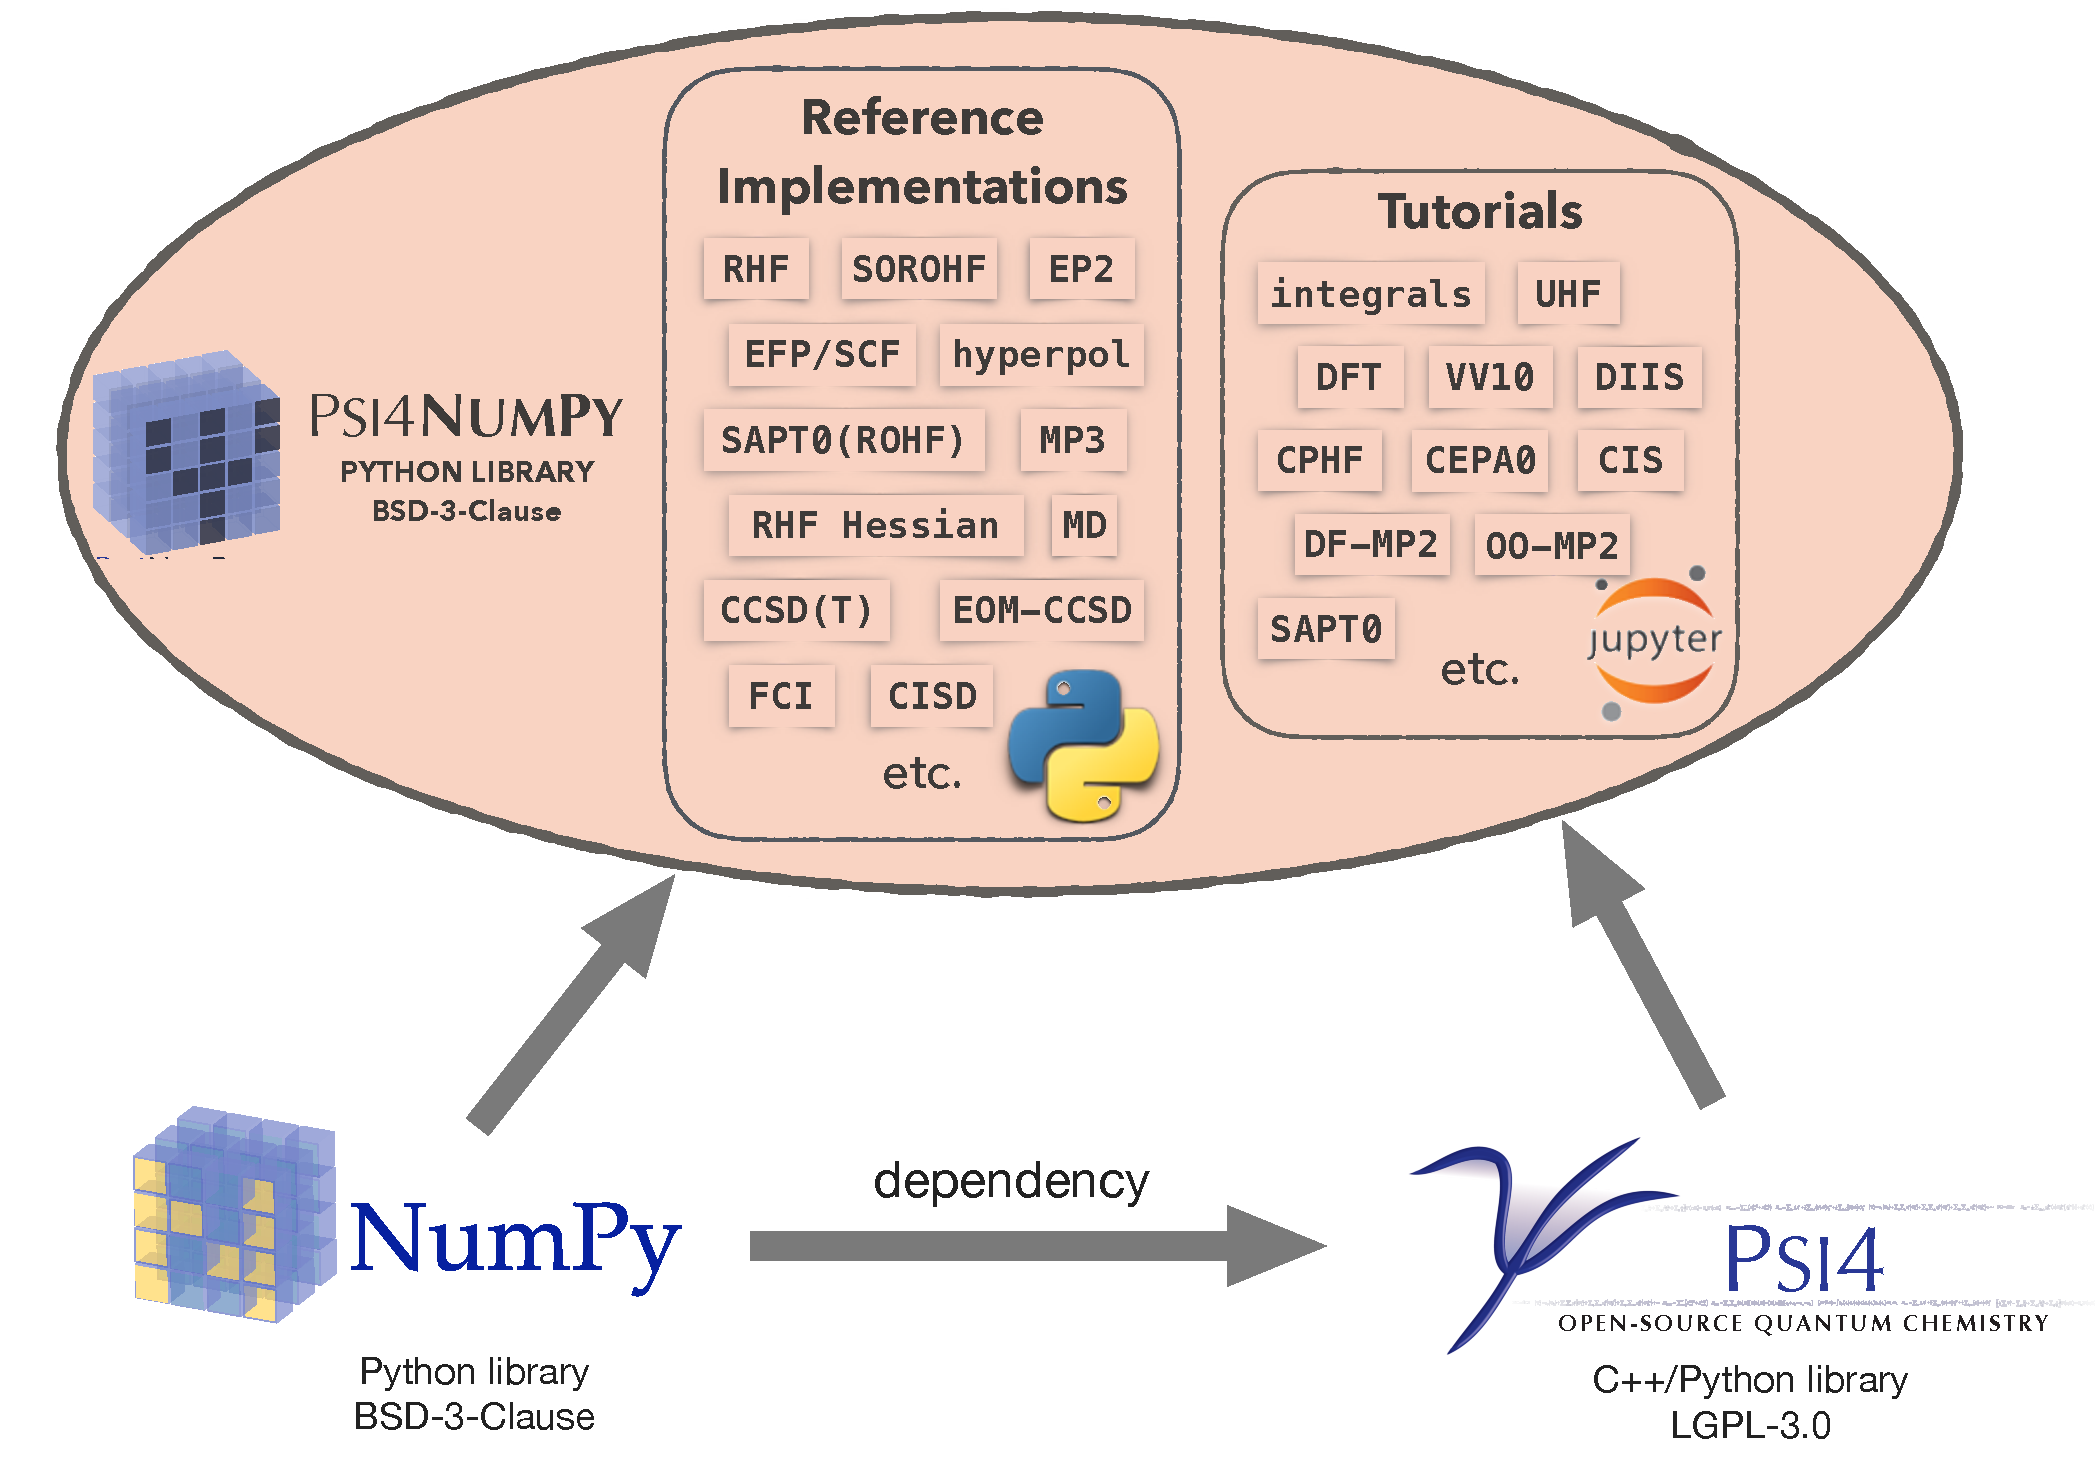
\includegraphics[width=\linewidth,keepaspectratio]{./figures/psi4numpy_ecosystem2.pdf}
\end{frame}

\begin{frame}
  \frametitle{\pfn{} is an ideal platform for teaching about \textit{ab initio} spectroscopy}
\end{frame}

\begin{frame}
  \frametitle{Jupyter Notebooks allow mixing of concepts, equations, and code in an exploratory environment}
\end{frame}

\begin{frame}
  \frametitle{\pfn{} is welcoming to external contributors}
\end{frame}

\begin{frame}
  \frametitle{Future extensions}
\end{frame}

\begin{frame}
  \frametitle{Conclusions}
\end{frame}

\begin{frame}
  \frametitle{Acknowledgments}
\end{frame}

\begin{frame}
  \frametitle{Thank you}
\end{frame}

\appendix

\begin{frame}
  \frametitle{LR(MI) is BSSE-free by construction}
\end{frame}

\immediate\closeout\tempfile

\end{document}
